\chapter{Paketeinteilung und Klasseninteraktion}

\section{App}

\subsection{User Interface Layer} 

\subsection{View}

\begin{figure}[H]
	\centering
	\includegraphics[width=1\textwidth]{pics/viewPackages/ViewPaketmodel.pdf}%
	\caption{Einzelne Pakete des User Interface Layers}%
	\label{view}%
\end{figure}

Die in Abbildung \ref{view} gezeigten Klassen sind die Klassen der View.
Die View erhält die Benutzereingabe direkt. Die grafische Oberfläche besteht aus einer Hauptaktivität, auch MainActivity, die durch ein Menü Fragments aufrufen kann. Das Menü ist ein eigenes Fragment, welches in der Toolbar der MainActivity zu sehen ist (mehr dazu in Kapitel 5.1). Die Fragments sind Klassen, denen .xml-Dateien zugeordnet sind und die die verschiedenen Oberflächen darstellen.

Abbildung \ref{viewinteract} zeigt einen groben Überblick über die Interaktion zwischen allen Fragments und der MainActivity. Die Pfeile zwischen den Fragments zeigen an, welche Fragments uni- oder bidirektionale Aufrufe aufeinander haben. Da das Menü in der Toolbar stets sichtbar ist, gibt es von jedem Fragment auch eine Interaktion "`Menü öffnen"', welche in \ref{viewinteract} im Sinne der Übersichtlichkeit nicht extra dargestellt wird. 
Was ebenfalls nur exemplarisch modelliert ist, ist der "`Zurück"'-Button des Smartphones, über den jedes Fragment verlassen werden kann. Nutzt man den "`Zurück"'-Button, gelangt man zurück auf das vorher angezeigte Fragment. Gibt es kein vorheriges Fragment mehr, weil man auf der Startseite der App ist, verlässt man die App mit dem Button.
Folgende Grafiken beschreiben nun genauer die Interaktionen zwischen den Fragments.

\begin{figure}[H]
	\centering
	\includegraphics[width=1\textwidth]{pics/viewPackages/ViewPaketmodel_Interaktion.pdf}%
	\caption{Interaktion zwischen den Fragments und der Main-Activity}%
	\label{viewinteract}%
\end{figure}

\subsubsection{FriendFragment Paket}
\begin{figure}[H]
	\centering
	\includegraphics[width=0.8\textwidth]{pics/viewPackages/FriendFragmentPaket.pdf}%
	\caption{FriendFragment Paket}%
	\label{view}%
\end{figure}


Das FriendFragmentPaket ist dafür zuständig, die graphischen Oberflächen der Freunde- und Gruppenverwaltung zu erstellen. 
Sowohl die Übersicht über die Gruppen eines Nutzers, als auch die Liste der Freunde eines Nutzer haben einen eigenen Menüpunkt, deswegen sind diese Fragments über das Appmenü erreichbar.


\subsubsection{RecipeFragment Paket}
\begin{figure}[H]
	\centering
	\includegraphics[width=0.8\textwidth]{pics/viewPackages/RecipeFragmentPaket.pdf}%
	\caption{RecipeFragment Paket}%
	\label{view}%
\end{figure}

Das RecipeFragmentPaket ist dafür zuständig die graphischen Oberflächen der Rezeptansichten. 
Wichtig ist die Unterscheidung von öffentlichen und privaten Rezepten. Öffentliche Rezepte haben ein festes Format und haben kein einziges Attribut = null , wobei private Rezepte nicht formatiert sein müssen und leere Attribute haben können. Daher ist die Anzeige der zwei Rezepttypen verschieden. 
Das RecipeListFragment stellt eine Liste der privaten Rezepte eines Autors dar. Es kann über das Appmenü aufgerufen werden.

\subsubsection{ProfileFragment Paket}
\begin{figure}[H]
	\centering
	\includegraphics[width=0.8\textwidth]{pics/viewPackages/ProfileFragmentPaket.pdf}%
	\caption{ProfileFragment Paket}%
	\label{view}%
\end{figure}

Das ProfileFragment Paket ist dafür zuständig, eine Graphische Oberfläche für die Nutzerverwaltung bereitzustellen. 
Ein angemeldeter Nutzer kann über das Appmenü das eigene Profil aufrufen. Dann wird das ProfileDisplayFragment angezeigt. Über den "`Bearbeiten"'-Button kommt der Nutzer auf das ProfileEditFragment seines Profils. Möchte er sein Passwort ändern, kann er über den "`Login-Daten ändern"'-Button das ChangePasswordFragment öffnen, um das zu tun.
Das LoginFragment ist über das Appmenü erreichbar. Über den "`Registrieren"'-Button gelangt man auf das RegistrationFragment. Hat sich in diesem Fragment ein Nutzer registriert und klickt auf den "`Registrieren"'-Button, wird er auf das ProfileDisplayFragment seines neu erstellten Profils geleitet.


\subsubsection{SearchFragment Paket}
\begin{figure}[H]
	\centering
	\includegraphics[width=0.8\textwidth]{pics/viewPackages/SearchFragmentPaket.pdf}%
	\caption{SearchFragment Paket}%
	\label{view}%
\end{figure}
Das SearchFragment Paket ist dafür zuständig die 
graphische Oberfläche für die verschiedenen Suchfunktionen
bereit zu stellen. 

\subsubsection{ShoppingListFragment Paket}
\begin{figure}[H]
	\centering
	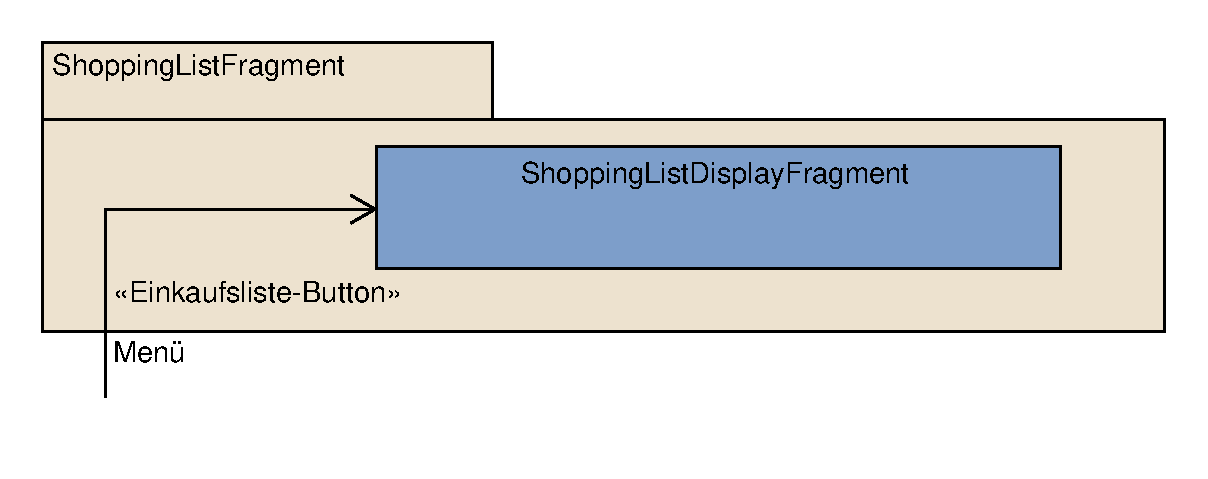
\includegraphics[width=0.8\textwidth]{pics/viewPackages/ShoppinglistFragmentPaket.pdf}%
	\caption{ShoppinglistFragment Paket}%
	\label{view}%
\end{figure}

Das ShoppingListFragment Paket ist dafür zuständig, die Oberfläche
der Einkaufsliste darzustellen. Das Fragment ist über das Appmenü erreichbar.


\subsubsection{FeedFragment Paket}
\begin{figure}[H]
	\centering
	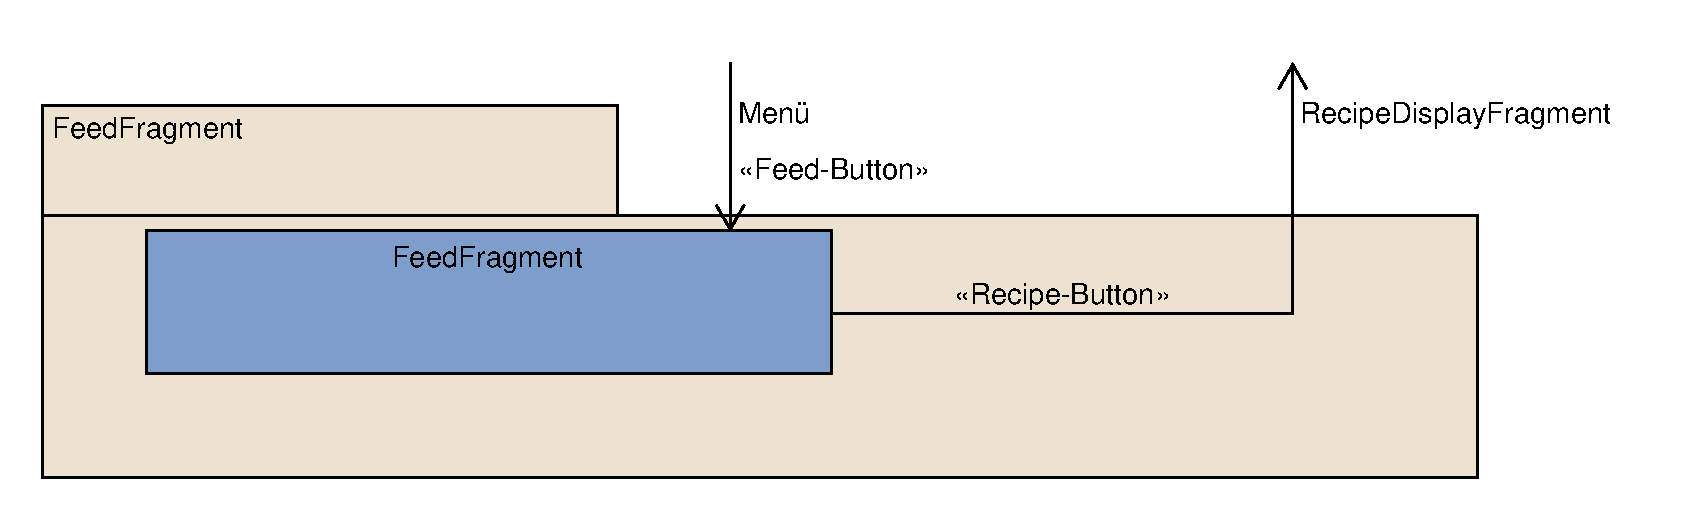
\includegraphics[width=\textwidth]{pics/viewPackages/FeedFragmentPaket.pdf}%
	\caption{FeedFragment Paket}%
	\label{view}%
\end{figure}
Das FeedFragment Paket ist dafür zuständig, die Oberfläche
des Feeds darzustellen. Wenn diese Funktionalität implementiert ist, ist der Feed die Startseite der App und durch das Appmenü erreichbar. Klickt ein User auf einen der Buttons im Feed, so wird er auf das entsprechende Rezept geleitet und das RecipeDisplayFragment öffnet sich.

\subsubsection{FavouriteFragment Paket}
\begin{figure}[H]
	\centering
	\includegraphics[width=\textwidth]{pics/viewPackages/FavouriteFragmentPaket.pdf}%
	\caption{FavouriteFragment Paket}%
	\label{view}%
\end{figure}

Das FavouriteFragment Paket ist dafür zuständig, die Oberfläche
der Favoritenliste darzustellen.
Diese hat einen eigenen Punkt im Appmenü und ist somit von diesem aus erreichbar. Verlassen wird das Fragment entweder über den "`Zurück"'-Button, oder, indem der Nutzer auf ein angezeigtes Rezept in der Favoritenliste klickt. Dann wird das RecipeDisplayFragment geöffnet.

\subsubsection{AddEditCommentFragment Paket}
\begin{figure}[H]
	\centering
	\includegraphics[width=\textwidth]{pics/viewPackages/CommentFragmentPaket.pdf}%
	\caption{FavouriteFragment Paket}%
	\label{view}%
\end{figure}
Das AddEditCommentFragment Paket ist dafür zuständig, die Oberfläche
der Kommentarbearbeitung darzustellen. Das Fragment wird aufgerufen, wenn im RecipeDisplayFragment ein angemeldeter Nutzer bei einem seiner eigens erstellten Kommentare auf "`bearbeiten"' drückt, oder wenn ein angemeldeter Nutzer auf den "`Kommentar schreiben"'-Button drückt. 
Wird der "`kommentieren"'-Button gedrückt, so wird das vorherige RecipeDisplayFragment wieder angezeigt.

\subsubsection{AdminFragment Paket}
\begin{figure}[H]
	\centering
	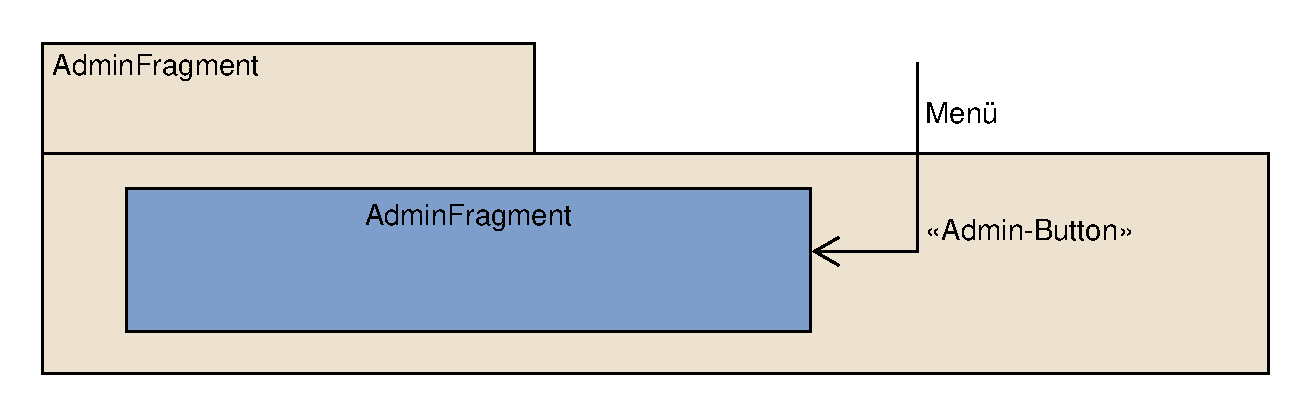
\includegraphics[width=\textwidth]{pics/viewPackages/AdminFragmentPaket.pdf}%
	\caption{AdminFragment Paket}%
	\label{view}%
\end{figure}
Das AdminFragment Paket ist dafür zuständig, die Oberfläche
des Admins darzustellen. Über diese hat der Admin die Möglichkeit gemeldete Rezepte, Nutzer, oder Gruppen manuell zu überprüfen und zu entfernen. Ist ein Nutzer als Admin angemeldet, so ist dieses Fragment über das Appmenü aufrufbar.


\subsection{ViewModel}

\begin{figure}[H]
	\centering
	\includegraphics[width=\textwidth]{pics/viewModel/ViewModelPackages.pdf}%
	\caption{Die Packages mit enthaltenen ViewModel-Klassen}%
	\label{vmpackages}%
\end{figure}

An sich sieht das ViewModel-Paket von der Struktur her analog so aus, wie die View-Struktur, da jedes Fragment ein ViewModel benötigt. Das SearchWithTagsFragment ist die einzige Ausnahme, da es von zwei verschiedenen Fragments aus aufgerufen wird und deswegen unterschiedlicher Funktionalitäten bedarf (mehr dazu in Kapitel 5.2). Was auch anders ist, sind die Verbindungen. Die ViewModels haben untereinander keinerlei Interaktion, sondern geben Daten und Anfragen durch Befehle an das Repository zu den Datenquellen durch. Jede VM-Klasse hat also eine Verbindung zum Repository.

\subsection{Domain Layer}

\subsubsection{Domain Entities}

\begin{figure}[H]
	\centering
	\includegraphics[width=\textwidth]{pics/EntityPackage.pdf}%
	\caption{Das Domain Entity-Paket mit Klassen}%
	\label{domain}%
\end{figure}

Die Domain Entities stellen auf der Appseite den Kern des Models dar. Sie liegen in einem Paket und interagieren miteinander, aber nicht mit Klassen außerhalb ihres Paketes. Die Interaktion der Entities ist in Kapitel 6.1 ausführlicher erklärt.

\subsubsection{Domain Layer Interfaces}

\begin{figure}[H]
	\centering
	\includegraphics[width=\textwidth]{generatedpics/DomainLayerInterfaces.pdf}%
	\caption{Die Interfaces des Domain Layers}%
	\label{interf}%
\end{figure}

Im Domain Layer liegen einige Interfaces, die für verschiedene Funktionalitäten gebraucht werden. Unter anderem sind die Repository-Interfaces, das ImportExport-Interface und das Authentifizierungs-Interface hier enthalten. Diese bieten Schnittstellen, um Bibliotheken oder eigene Funktionale Klassen (zB. das Repository) gekapselt einzubinden.
Im Repository-Interfaces-Package sind verschiedene Interfaces enthalten. Für jede Klasse im Repository (siehe folgenden Abschnitt), ist ein Interface im Package enthalten, welches die Methoden und Attribute der Klasse vorgibt.

\subsection{Data Layer}

\begin{figure}[H]
	\centering
	\includegraphics[width=\textwidth]{generatedpics/RepositoryPackage.pdf}%
	\caption{Das Paket mit Klassen des Repositories}%
	\label{repo}%
\end{figure}

Das Repository enthält für fast jede Domain Entity eine Klasse, in der Methoden zur Datenverwaltung dieser Entity enthalten sind. Es ist aufgeteilt in ein Package für die lokale SQLite Room-Datenbank und eines für den Webserver.

\section{Server}

\subsection{Api und Model Pakete}

In der Abbildung \ref{serverapidb} werden alle Pakete und Klassen aufgelistet, welche für die Kommunikation mit den Clients (Api/Controller), behandeln von den Anfragen (Services) und den Zugriff auf die Datenbank (Dao und Model) zuständig sind. Die DTOs sind die Klassen bzw. Objekte, welche über das Netzwerk zwischen Client und Server versendet werden.

\begin{figure}[H]
	\centering
	\includegraphics[width=\textwidth]{pics/PacketServerApi_and_Db.pdf}%
	\caption{Die Packages und Klassen für die ServerApi und die Anbindung an die Datenbank}%
	\label{serverapidb}
\end{figure}

\subsection{Konfiguration- und Ausführungspakete}
In der folgenden Abbildung \ref{serverconfig} werden alle Pakete und Klassen aufgelistet, welche für das Konfigurieren, Starten von dem Server und Authentifizieren von Nutzern zuständig sind.\\
Das Paket Security beinhaltet Klassen, die für die Authentifizierung von Nutzern, die den Dienst anfragen, verwendet werden. Die Klassen verwenden Spring Boot Security und Firebase. Das Paket exzellenzkoch enthält nur die Klasse ExzellenzkochApplication. Diese Klasse enthält die Main-Methode und startet den Dienst. Die Konfigurationsklassen befinden sich im Paket config. In WebSecurityConfig wird die Konfiguration der Spring Boot Security festgelegt und in der Klasse FirebaseConfig die Konfigurationen für die Firbaseverbindung. Im Paket exceptions befinden eine Exceptionenklasse, welche geworfen wird, wenn eine Element in der Datenbank nicht gefunden wird.

\begin{figure}[H]
	\centering
	\includegraphics[width=\textwidth]{pics/PacketServerConfig.pdf}%
	\caption{Die Packages und Klassen für die Konfiguration und Ausführung des Servers und Authentifizierung von Nutzern}%
	\label{serverconfig}
\end{figure}

\subsection{Kommunikation zwischen Controllerpaket und Servicepaket}

\ref{kommContrServ} zeigt den Zugriff der Controller-Klassen auf die Service-Klassen. Jeder Controller greift auf seinen Service zu.

\begin{figure}[H]
	\centering
	\includegraphics[width=\textwidth]{pics/KommunikationServerControllerService.pdf}%
	\caption{Die Packages und ihre Klassen und die Kommunikation zwischen Service und Controller}%
	\label{kommContrServ}
\end{figure}

\subsection{Kommunikation zwischen Servicepaket und Daopaket}

In \ref{kommServDao} wird der Zugriff der Service-Klassen auf die Dao-Klassen abgebildet. Ein Service kann auf verschiedene Dao zugreifen und ein Dao wird auch von verschiedenen Service-Klassen verwendet.

\begin{figure}[H]
	\centering
	\includegraphics[width=\textwidth]{pics/KommunikationServerServiceDao.pdf}%
	\caption{Die Packages und ihre Klassen und die Kommunikation zwischen Services und Dao}%
	\label{kommServDao}
\end{figure}


